\documentclass{school-22.211-notes}
\date{February 13, 2012}

\begin{document}
\maketitle


%%%%%%%%%%%%%%%%%%%%%%%% Neutron Slowing Down and Thermalization %%%%%%%%%%%%%%%
\lecture{Neutron Slowing Down and Thermalization}

\topic{Summary: Reuss Ch 7 Neutron Slowing Down}
\begin{enumerate}
\item Decouple absorption and scattering is possible because absorption is complicated at lower energies, whereas scattering is the opposite (b/c inelastic and anisotropic aspects). 

\item Elastic vs inelastic: elastic scattering has no threshold, making it the most important one in neutron slowing down. 

\item Laws of elastic collision: 
  \begin{align}
    \frac{E_{nf}}{E_{ni}} &= \frac{A^2 + 1 + 2A \cos \theta}{(A+1)^2} = \frac{1}{2} \left( 1 + \alpha + (1-\alpha) \cos \theta \right) \\
    \cos \psi &= \frac{1 + A \cos \theta}{\sqrt{A^2 + 1 + 2A \cos \theta}} \\
    \alpha &= \frac{(A-1)^2}{(A+1)^2} = \mbox{min ratio between final n energy and initial} 
  \end{align}

\item Lethargy, a unitless measurement of energy:
  \eqn{ u = \ln \frac{E_{\mathrm{ref}}}{E} }
Notice as time goes, neutrons slow down, $u$ increases, making it like a measure of the age of the neutrons. Then we can write:
\begin{align}
w &= u_f - u_i = -\ln \left( \frac{1}{2} ( 1 + \alpha + (1-\alpha) \cos \theta ) \right) \\
w_{min} &= 0 \\
w_{max} &= \epsilon = -\ln \alpha \\
P(w) \dw &= \frac{e^{-w}}{1 - \alpha} \dw \\
\expect{w} &= \xi = 1 - \frac{\alpha \epsilon}{1 - \alpha} 
\end{align}
$\xi$ is the average `progress' of the neutrons in terms of lethargy on the path of slowing down. That is, neutrons advance by $\xi$ lethargy units on average at each collision. Then to overcome the total lethargy interval $U = \ln \frac{E_0}{E_1}$, the number of collisions needed is:
\eqn{ n = \frac{U}{\xi} }

\item Moderating power is the best measure of a material's ability to slow down neutrons. It has two forms:
\eqn{\mbox{per atom basis} = \xi \sigma_s \fsp \fsp \fsp \mbox{per volume basis} = \xi \Sigma_s   }
A good moderating material should have: high slowing down (hence light nuclei), low capture (D, Be, C), moderating power (take into account both high slowing down and high scattering xs). 

\item Laws of inelastic collision. Elastic scattering is important for moderators because they are light; inelastic scattering is important for heavy materials like the fuel because they have almost no elastic collision. Minimum energy of the neutron for an inelastic collision is:
\eqn{ E_{\mathrm{threshold}} = \frac{A+1}{A} Q } 

\item First form of the slowing down equation:
  \begin{align}
    \rho(u) \du 
    &= \mbox{arrival density} = \begin{array}{l}
      \mbox{\# neutrons arriving per time and per volume} \\
      \mbox{in d$u$ between $u$ and $u + \du$ following a scattering to $u'$} 
      \end{array} \\
    &= \overbrace{\int_{-\infty}^u \Sigma_s (u') \Phi(u') \du'}^{\textcircled{1}} \overbrace{ P(u'\to u) \du }^{\textcircled{2}} \\
    \textcircled{1} &= \mbox{\# neutrons travelling in du' and scattered per time and per volume} \\
    \textcircled{2} &= \mbox{probability a neutron scattered at u' will be transferred in du} \\
    \rho(u) &= \int_{-\infty}^u \Sigma_s (u'\to u) \phi(u') \du' \\
    S(u) + \rho(u) &= \boxed{S(u) + \int_{-\infty}^u \Sigma_s (u'\to u) \phi(u') \du  = \Sigma(u) \phi(u) }
  \end{align}
\end{enumerate}

%%%%%%%%%%%%%%%%%%%%%%%%%%%% Ch 9 %%%%%%%%%%%%%%%%%%%%%%%%%%%%%%%%
\topic{Summary: Reuss Ch 9 Thermalisation of Neutrons (need completion)}


\topic{Developing An Infinite-medium Monte Carlo Neutronics}
*does xs depend on geometry? if not, why does it matter infinite medium? 

\subtopic{Isotopic Importance by Infinite Medium Reactor Materials}

\begin{table}
  \centering
  \begin{tabular}{|c|c|c|}
    PWR & & \\
    BWR & & 
  \end{tabular}
  \caption{Volume Fraction of Reactor Materials}
\end{table}
Notice in PWR, H and O densities come out to be the same. 

Usually given a xs, it is given in 0.025 eV because it is the peak of the Maxiwillean distribution in room temperature. 

\subtopic{Absorption and Scattering}
Absorption and scattering always line up together in terms of energy. 

Sodium has a high capture xs in thermal range, and a small capture xs in fast range. But we can still build a thermal reactor with water as moderator and sodium as coolant, as long as sodium's volume is lower than that of the H. 

\topic{Models for High Energy Elastic Scattering Physics}
Compression: log slowing down. 

Take an energy and adds up all the neutrons in that energy, we get flux vs. energy. 

\subtopic{Flux vs. energy graph}
The curve due to Placzek Transients; if the lower energy bound is not low enough, the flux would tail down, which means that we are not tracking enough energy. WIth enough energy, the flux should be a $\frac{1}{E}$ shape. 

\subtopic{Flux vs. lethargy}
 calculate mean energy and place them in corresponding bins; even at higher generations, there are still some neutrons not slowed down entirely yet, so the flux curve tails down. In lethargy space, $\phi(E)$ should be constant. 

Binning method: When we are plotting, we are really plotting the expectation value of the numbers of neutrons; so if we ask `how many neutrons would there be at x energy level' the answer should be zero. So the bins have to be fine enough to see the details, but not too fine that the bins got no more neutrons. 


\topic{Models for Fission Neutron Emission Spectra}
When building a cdf for neutron emission, it is always important to sample right after and compare with the spectrum to make sure the cdf is correct. 

Spectrum: shape in energy, which is independent on the number of incoming neutrons and xs for one specie; for two species, the relative xs matter. 

Fission source peak: have to take into account the cross section: 
\eqn{\phi(E) \propto \Sum_N \Sum_g N_g^n \tau_g^n = \Sum_n \Sum_g N_g^n \frac{1}{\Sigma(E_g^n)}   }
So without taking into account xs, the sudo flux is flat and missing the fission source peak; taking into account hygrogen peak xs, the real flux peaks shows up. 

\topic{Models for Equilibrium Thermal Scattering Physics}
\subtopic{Equilibrium Monatomic Gas: Maxwellian Distribution of Target Energy}

Maxiwellian: 4 eV cut-off. 


Adding thermalization into the hydrogen flux, we get the bump. The size of the bump depends on the absorber. If we add a $1/v$ absorber with a 0.2 absorption-to-scattering ratio at 0.025 MeV, then the flux in hydrogen looks more like the flux in a typical LWR. 


\subtopic{U238 Target in Motion Thermal Scattering Distributions}
Fuel in LWR is around 1000K. Assume 1200K for now, then the four times cut-off for a 25 kT (2.5 eV) neutron has a cutoff of 200 kT (20 eV). 

Scattering resonance: anti-resonance, due to the interacting wave between potential scattering and compound nuclear scattering. 

The problem is, the scattering xs goes to 0 and goes up (scattering may even be larger than absorption) right around the peak energy, and if you cutoff right before the peak, the results are wrong. 

\subtopic{Bound Elastic Scattering of H in Water Molecule vs Temperature}
So far we've only talked about free gas; in the case of tightly bound atoms at very low wnergy, 
\eqn{\sigma_{\mathrm{bound}} = \left( 1 + \frac{1}{A} \right) \sigma  }
The dependency on $A$ suggests that the bound elastic scattering matters for light nuclei, and not so much for heavy nuclei. 

In the case of hydrogen, the free gas model would still provide the right shape, but the probability can be off by a factor of 10. In the case of graphite, the free gas model does not provide the right shape. The lower energy you want to go, the more careful you need to be. 

Know the terminologies $S, \alpha$ (momentum transfer), $\beta$ (energy transfer). 

A couple of important points:
\begin{itemize}
\item Thermal scattering distributions: generate cdf for 1kT, 4kT, 8kT.  
\item 4 eV is the typicall up-scattering cutoff energy in many models and codes. For an incident neutron energy higher than 4 eV, use asymptotic elastic down scattering. 
\end{itemize}

\topic{HW2: Slowing Down with Maxwellian Free Gas Thermalization}
For HW2, we place a $1/v$ absorber in the thermal range, because otherwise the up-scattering would push neutrons to higher energies infinitely. For the $1/v$ absorber, we set the xs at 0.025 eV to a certain number (like 7 barns), and set the xs from 10e-3 eV upto a certain energy to be $\sigma_{0.025} \sqrt{\frac{E_{0.025}}{E}}$. 7 barns is picked for absorption xs because H's scattering xs is about 11 barns, and this way the absorption-to-scattering ratio is something around 20\%. The result of my HW2 is shown in Figure~\ref{pset2}.
\begin{figure}
  \centering
  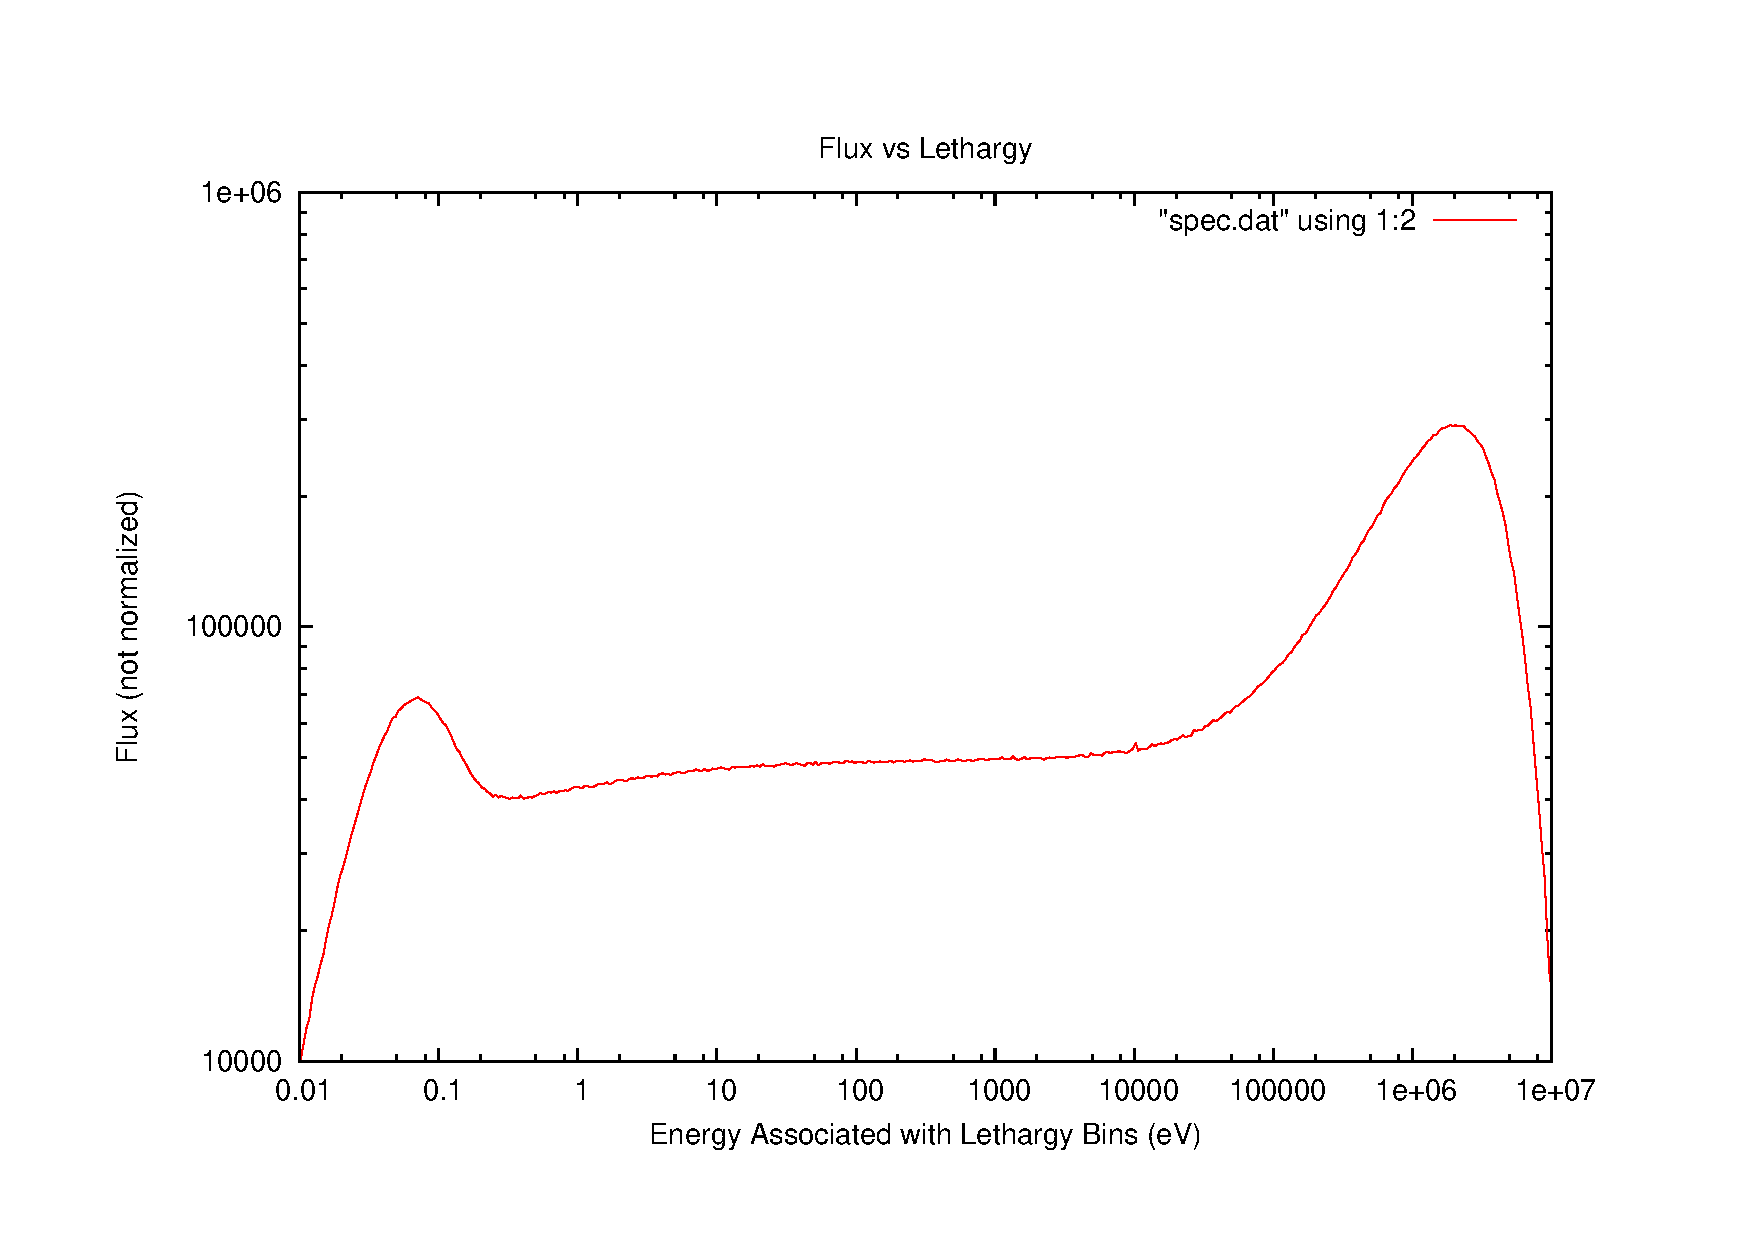
\includegraphics[width=4in]{images/spec.uncrop.pdf}
  \caption{Slowing Down with Maxwellian Free Gas Thermalization} \label{pset2}
\end{figure}


\end{document}
